%%==================================================================%%
%% Author : Sa�udo Olmedo, Ignacio                                  %%
%%          S�nchez Barreiro, Pablo                                 %%
%% Version: 1.2, 18/06/2014                                         %%
%%                                                                  %%
%% Memoria del Proyecto Fin de Carrera                              %%
%% Planificacion/CasoEstudio                                        %%
%%==================================================================%%

\begin{figure}[!tb]
  \centering
  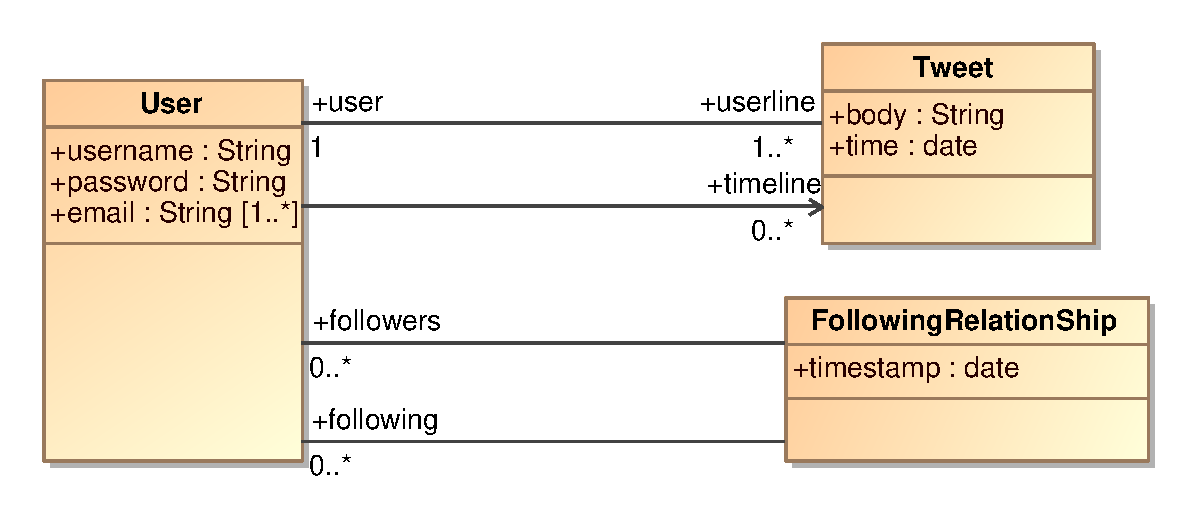
\includegraphics[width=.8\linewidth]{m2m/images/twissandra.eps} \\
  \caption{Modelo UML Twissandra}
  \label{back:fig:twissandra}
\end{figure}

En esta secci�n se presenta el caso de estudio que se analizar� lo largo de este proyecto. El caso de estudio que se analizara trata sobre Twissandra, Twissandra es un proyecto creado para aprender como utilizar Cassandra. El modelo UML correspondiente a Twissandra se puede ver en la figura~\ref{back:fig:twissandra}.

Twissandra es una versi�n simplificada de Twitter, que es a menudo utilizada para demostrar las capacidades de Cassandra. Twitter es una red social muy conocida que permite escribir a los usuarios peque�os mensajes de texto, funciona de la siguiente manera: los usuarios registrados pueden publicar tweets. Un tweet es simplemente un texto con un l�mite de 140 caracteres publicado a una hora determinada. La colecci�n de todos los tweets publicados por un usuario cronol�gicamente ordenados, est�n asignados a su Userline.
Cada usuario registrado en Twissandra puede seguir a otros usuarios registrados. Cuando decimos que Pedro sigue a Mar�a significa que Pedro est� interesado en saber qu� publica Mar�a en su tabl�n, por lo que Pedro recibir� todos los mensajes que publique Mar�a en su tabl�n. As�, cada usuario registrado tiene tambi�n un timeline que vendr�a a ser la colecci�n de todos los tweets de las personas a las que sigue ordenadas cronol�gicamente.

Los principales casos de uso de un sistema de este tipo son: (1) obtener el timeline de un usuario determinado; (2) obtener el Userline de un usuario, (3) obtener la lista de usuarios que un usuario est� siguiendo; y (4) obtener la lista de usuarios que est�n siguiendo a un usuario espec�fico. Estas dos �ltimas listas deben ser ordenadas cronol�gicamente.

Una vez entendido en los siguientes cap�tulos se procede a detallar el proceso de creaci�n de un generador de c�digo de este caso de estudio. 